
\section{Sistemas de control de versiones locales} 
Un método de control de versiones usado por mucha gente es copiar los archivos a otro directorio (quizás indicando la fecha y hora en que lo hicieron, si son avispados). Este enfoque es muy común porque es muy simple, pero también tremendamente propenso a errores. Es fácil olvidar en qué directorio te encuentras, y guardar accidentalmente en el archivo equivocado o sobrescribir archivos que no querías.

\begin{itemize}
	\begin{center}
	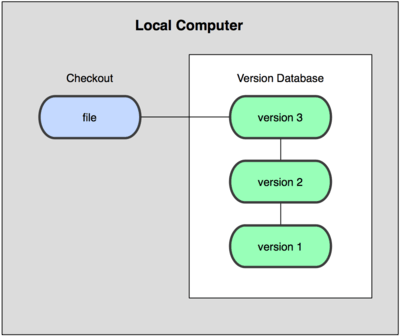
\includegraphics[width=14cm]{./Imagenes/imagen3} 
	\end{center}

	\item Una de las herramientas de control de versiones más popular fue un sistema llamado rcs, que todavía podemos encontrar en muchos de los ordenadores actuales. Hasta el famoso sistema operativo Mac OS X incluye el comando rcs cuando instalas las herramientas de desarrollo. Esta herramienta funciona básicamente guardando conjuntos de parches (es decir, las diferencias entre archivos) de una versión a otra en un formato especial en disco; puede entonces recrear cómo era un archivo en cualquier momento sumando los distintos parches.



\end{itemize} 